% !TeX program = pdfLaTeX
\documentclass[smallextended]{svjour3}       % onecolumn (second format)
%\documentclass[twocolumn]{svjour3}          % twocolumn
%
\smartqed  % flush right qed marks, e.g. at end of proof
%
\usepackage{amsmath}
\usepackage{graphicx}
\usepackage[utf8]{inputenc}

\usepackage[hyphens]{url} % not crucial - just used below for the URL
\usepackage{hyperref}
\providecommand{\tightlist}{%
  \setlength{\itemsep}{0pt}\setlength{\parskip}{0pt}}

%
% \usepackage{mathptmx}      % use Times fonts if available on your TeX system
%
% insert here the call for the packages your document requires
%\usepackage{latexsym}
% etc.
%
% please place your own definitions here and don't use \def but
% \newcommand{}{}
%
% Insert the name of "your journal" with
% \journalname{myjournal}
%

%% load any required packages here



% Pandoc citation processing
\newlength{\csllabelwidth}
\setlength{\csllabelwidth}{3em}
\newlength{\cslhangindent}
\setlength{\cslhangindent}{1.5em}
% for Pandoc 2.8 to 2.10.1
\newenvironment{cslreferences}%
  {}%
  {\par}
% For Pandoc 2.11+
\newenvironment{CSLReferences}[2] % #1 hanging-ident, #2 entry spacing
 {% don't indent paragraphs
  \setlength{\parindent}{0pt}
  % turn on hanging indent if param 1 is 1
  \ifodd #1 \everypar{\setlength{\hangindent}{\cslhangindent}}\ignorespaces\fi
  % set entry spacing
  \ifnum #2 > 0
  \setlength{\parskip}{#2\baselineskip}
  \fi
 }%
 {}
\usepackage{calc} % for calculating minipage widths
\newcommand{\CSLBlock}[1]{#1\hfill\break}
\newcommand{\CSLLeftMargin}[1]{\parbox[t]{\csllabelwidth}{#1}}
\newcommand{\CSLRightInline}[1]{\parbox[t]{\linewidth - \csllabelwidth}{#1}\break}
\newcommand{\CSLIndent}[1]{\hspace{\cslhangindent}#1}

\usepackage{hyperref}
\usepackage{amsmath}
\usepackage{amssymb}
\usepackage{bm}
\usepackage{natbib}
\usepackage{xcolor}
\usepackage{booktabs}
\usepackage{longtable}
\usepackage{array}
\usepackage{multirow}
\usepackage{wrapfig}
\usepackage{float}
\usepackage{colortbl}
\usepackage{pdflscape}
\usepackage{tabu}
\usepackage{threeparttable}
\usepackage{threeparttablex}
\usepackage[normalem]{ulem}
\usepackage{makecell}
\usepackage{xcolor}

\begin{document}

\title{Landscape floral resources provided by rapeseed correlate with
next-year solitary bee reproduction in a national participatory
monitoring program \thanks{Grants or other notes about the article that
should go on the front page should be placed here. General
acknowledgments should be placed at the end of the article.} }


    \titlerunning{Landscape floral resources correlate with next-year
solitary bee reproduction}

\author{  Victor Van der Meersch \and  Olivier Billaud \and  Magali San
Cristobal \and  Aude Vialatte \and  Emmanuelle Porcher \and  }

    \authorrunning{ Van der Meersch et al. }

\institute{
        Victor Van der Meersch \at
     Centre d'Ecologie et des Sciences de la Conservation (CESCO),
Muséum National d'Histoire Naturelle, Centre National de la Recherche
Scientifique, Sorbonne Université, Paris, France \\
     %  \\
%             \emph{Present address:} of F. Author  %  if needed
    \and
        Olivier Billaud \at
     Centre d'Ecologie et des Sciences de la Conservation (CESCO),
Muséum National d'Histoire Naturelle, Centre National de la Recherche
Scientifique, Sorbonne Université, Paris, France \\
     %  \\
%             \emph{Present address:} of F. Author  %  if needed
    \and
        Magali San Cristobal \at
     Dynamique et Ecologie des Paysages Agriforestiers (DYNAFOR),
Institut national de recherche pour l'agriculture, l'alimentation et
l'environnement, Université de Toulouse, Castanet Tolosan, France \\
     %  \\
%             \emph{Present address:} of F. Author  %  if needed
    \and
        Aude Vialatte \at
     Dynamique et Ecologie des Paysages Agriforestiers (DYNAFOR),
Institut national de recherche pour l'agriculture, l'alimentation et
l'environnement, Université de Toulouse, Castanet Tolosan, France \\
     %  \\
%             \emph{Present address:} of F. Author  %  if needed
    \and
        Emmanuelle Porcher \at
     Centre d'Ecologie et des Sciences de la Conservation (CESCO),
Muséum National d'Histoire Naturelle, Centre National de la Recherche
Scientifique, Sorbonne Université, Paris, France \\
     \email{\href{mailto:emmanuelle.porcher@mnhnfr}{\nolinkurl{emmanuelle.porcher@mnhnfr}}}  %  \\
%             \emph{Present address:} of F. Author  %  if needed
    \and
    }

\date{Received: date / Accepted: date}
% The correct dates will be entered by the editor


\maketitle

\begin{abstract}
Wild bees depend on floral resources available in the landscape, partly
provided by mass flowering crops (MFCs), such as rapeseed or sunflower.
To understand whether and to what extent these crops could help maintain
bee populations on the long term, we investigated the inter-annual
impact of MFC resources on solitary bee reproduction. We studied a large
standardized citizen science dataset, in which farmers collected data on
the the abundance of mud-sealed tubes in trap nests, between 2012 and
2017, in nearly 600 fields distributed across France. We modelled the
relation between bee nesting and landscape resources of the current and
previous year, also taking local farming practices into account
(conventional vs.~organic farming). Solitary bee reproduction was
positively correlated with the quantity of floral ressources provided by
rapeseed cultivated the year preceding observations. Reproduction was
also positively linked to the area of permanent meadows. On the
contrary, we found a weakly significant negative relationship between
sunflower cultivated the year preceding observations and bee
reproduction. Our models also confirm that local practices should be
taken into account when assessing the influence of landscape context,
even though their effects were more difficult to interpret. We therefore
show that solitary bee reproduction is likely to be positively and
durably affected by rapeseed cover. A moderate cover of rapeseed may
thus help to maintain solitary bee populations, in combination with
semi-natural habitats, which provide more diverse food and nesting
sites.
\\
\keywords{
        agriculture; \and
        biodiversity; \and
        citizen science; \and
        Osmia; \and
        solitary bees; \and
        pollination; \and
        floral ressource; \and
    }


\end{abstract}


\def\spacingset#1{\renewcommand{\baselinestretch}%
{#1}\small\normalsize} \spacingset{1}


\newpage

\hypertarget{intro}{%
\section{Introduction}\label{intro}}

Agriculture and biodiversity are inter-linked. The observed trend toward
the intensification of farming practices and the homogenization of
landscapes over the past decades have triggered significant negative
impacts on insect diversity and abundance (Benton et al. 2002;
Sánchez-Bayo and Wyckhuys 2019). In particular, pollinators are known to
decline because of several human-related drivers, including habitat loss
and use of agrochemicals (S. G. Potts et al. 2010; Vanbergen and the
Insect Pollinators Initiative 2013). This major loss of insects could
have negative effects on ecosystem functioning, as insects play a
central role in a variety of processes, including pollination: 80\% of
wild plants are estimated to depend on animals for pollination
(Ollerton, Winfree, and Tarrant 2011), and 35\% of global agricultural
production comes from crops that depends on pollinators (Klein et al.
2007). In turn, many pollinator species depend at least partially on
floral resources availability and accessibility (S. G. Potts et al.
2003). The spatial and temporal distribution of floral resources is
therefore essential for pollinators, especially for central place
foragers such as wild bees, which are not spared from human disturbances
(Biesmeijer et al. 2006; Goulson, Lye, and Darvill 2008; S. G. Potts et
al. 2010; Burkle, Marlin, and Knight 2013; Ben A. Woodcock et al. 2016)
and cannot follow the seasonality of flowering from one area to another.
They may be more efficient pollinators of wild plants and crops than
honey bees (Lucas A. Garibaldi et al. 2014; Mallinger and Gratton 2015),
and thus important for supporting pollinator-dependent crops and
sustaining pollination service in agricultural areas. (Steffan-Dewenter
and Leschke 2003; Pereira-Peixoto et al. 2014)

In agricultural landscapes, floral resources for pollinators are
provided both by wild plants and mass flowering crops (MFCs): the former
provide less abundant but more constant resources than crops, while the
latter provide massive amounts of resources but during a restricted
period of flowering. Although wild bees seem to depend more on wild
floral resources than on MFCs (Rollin et al. 2013), many of them,
including solitary bees, are still known to use MFCs (Jauker,
Bondarenko, et al. 2012; Le Féon et al. 2013). Besides, the balance
between positive and negative effects of MFCs on wild bees remains
unclear. On the one hand, MFCs provide both pollen and nectar resources
that positively affect solitary bee species richness (Diekötter et al.
2014), abundance (Le Féon et al. 2013; Riedinger et al. 2015) and
reproduction (Holzschuh et al. 2012; Jauker, Peter, et al. 2012), even
though some studies found a negative effect (Holzschuh et al. 2016; Shaw
et al. 2020). On the other hand, MFCs are often associated with
intensive agriculture, which comes with a simplification of landscapes,
including fewer semi-natural landscape elements providing cavities for
nesting, as well as more frequent use of pesticides, which may have
lethal and sublethal effects on solitary bees (Biddinger 2013; Artz and
Pitts-Singer 2015; Rundlöf et al. 2015; Sgolastra et al. 2017; Azpiazu
et al. 2019). Moreover, by favoring generalist pollinators, a high
proportion of MCF in the landscape may disrupt local plant-pollinator
interactions (Diekötter et al. 2010).

The observed contrasting relationships between MFCs and solitary bee
abundance or reproduction may be due in part to various source of
heterogeneity in the aforementioned studies, which we we aim to control
in the current study. First, these studies were performed in a variety
of contexts, in terms of landscape structure, farming practices or
climate. In order to generalize the actual role of MFCs, we here analyse
a unique dataset obtained across a wide range of agro-environmental
contexts. \emph{Another reason for the contrasting effects of MFCs on
wild bees may be related to the variety of ways both bee populations and
floral resources are characterized. To characterize bee populations, one
can measure either the presence of adults, using e.g.~pan traps, or
nesting activity, using trap nests.} {[}\textbf{Aude propose de
supprimer}{]} To characterize the effects of MFCs, most researches
studied either immediate impacts (MFCs generally attract bees, with
sometimes a positive effect on breeding, see Holzschuh et al. (2012), Le
Féon et al. (2013), and Diekötter et al. (2014)) or year-to-year effects
(MFCs may influence bee abundance the following year, see Jauker, Peter,
et al. (2012) and Riedinger et al. (2015)). The inter-annual effects of
MFCs on the fitness of wild bees populations is essential for their
maintenance on the long term. Understanding the balance between positive
effects (through the delivery of floral resources) and negative effects
(through possible pesticide contamination) according to
agro-environmental contexts is necessary to inform future
agro-ecological management of these crops. \emph{To our knowledge, few
studies have been conducted into the year-to-year impacts of MFCs on
wild bee populations, and they are often limited to a small number of
observations over relatively small areas.} {[}\textbf{Aude propose de
supprimer}{]}

This study investigates the relationship between the reproduction of
solitary bee populations and mass-flowering crop cover over a whole
country. Our goal is to complement previous studies, on the one hand by
examining year-to-year effects to assess the long term impact of MFCs,
and on the other hand by considering a broad area and a variety of
contexts. Our originality is to rely on a citizen science program with a
large number of sites (nearly 600 fields) all over France. We focus on
immediate and year-to-year landscape correlations with bee reproduction.
We aimed to assess whether the cover of two widespread MFCs (rapeseed
and sunflower) was correlated with solitary bee nesting both in the year
of monitoring and in the following year and thus might be able to
support bee populations through time.

\hypertarget{meth}{%
\section{Material and methods}\label{meth}}

\hypertarget{meth:1}{%
\subsection{Participatory monitoring of solitary bees in
fields}\label{meth:1}}

The study was conducted in fields monitored by farmers all over mainland
France between 2012 and 2017, within the framework of the Farmland
Biodiversity Observatory (FBO). The FBO targets several taxonomic groups
to identify farming practices and landscape elements that promote
farmland biodiversity (Billaud, Vermeersch, and Porcher 2020). To our
knowledge, this is one of the first national biodiversity monitoring
programs to use a participatory approach involving farmers. Over a total
of 1501 sites, we selected 576 sites, including 416 field crops and 166
meadows, for which all required environmental variables (see below),
including geographical coordinates, were well reported. Some sites were
monitored several years in a row (see below for more details).

\hypertarget{trap-nests-in-field-boundary}{%
\subsection{Trap nests in field
boundary}\label{trap-nests-in-field-boundary}}

All farmers set up two standardized trap nests 5 meter away in each
studied field boundary. A trap nest consisted of 32 cardboard tubes that
were fixed facing south, on a wooden post, 1 meter above the ground
(Billaud, Vermeersch, and Porcher 2020). Farmers monitored nest
occupancy, an indicator for bee reproductive performance, by counting
sealed tubes. They also reported a proxy for bee diversity by
identifying the sealing material (mud, chewed leaves, trichomes of wooly
plants\ldots). Theoretically, trap nests were meant to be monitored once
a month between March and November, but some observers tended to forget
some of the surveys. Within a year, 91.8\% of sites were sampled at
least twice, and 49\% at least five times. Accordingly, we did not
summarize data within a year, but chose to use all 3345 observations,
i.e.~one count in a given month per trap nest.

We focused our study on the most abundant category of sealing material,
i.e.~mud, which represents 65\% of observations. These mud-sealed tubes
are likely to be made mainly by \emph{Osmia} bees (Linsley 1958),
although some \emph{Megachile} may also use mud for nest building
(e.g.~subgenus \emph{Chalicodoma}, see Michener 2007).

\hypertarget{environmental-variables}{%
\subsection{Environmental variables}\label{environmental-variables}}

\hypertarget{landscape-variables}{%
\paragraph{Landscape variables}\label{landscape-variables}}

We used the national cartographic field registry (\emph{Registre
parcellaire graphique}, RPG) to map each crop type within a buffer
around each study site. We chose the size of the buffer \emph{a priori}
on the basis of ecological knowledge of solitary bees instead of testing
multiple spatial extents and taking the one that best predicts the
response, because the latter approach is sometimes biased (Jackson and
Fahrig 2015). The area of each crop in the buffer was calculated using
the R package \emph{sf} (Pebesma 2018).

We computed the area of the two main MFCs (rapeseed and sunflower) both
in the sampling year and the previous year. For the sampling year
calculation, we used a 250m-radius buffer since the distance at which
half of the population discontinues foraging (few hundred meters) is
more relevant than the species specific maximum foraging distance
(Zurbuchen et al. 2010). For the previous year calculation, we decided
to use a 1000m-radius buffer because the dispersal distance, from the
emergence site to the nesting site, is larger than the median foraging
distance of solitary bees. However, the choice of the buffer radius
(250m or 1,000m) for the area of MFCs the year preceding the observation
did not influence the results (not shown).

In order to take into account other floral resources and nesting
opportunities, we also computed the area of temporary meadows for both
sampling year and previous year, and the area of orchards and permanent
meadows in the sampling year only (because these land uses change little
through time). Finally, as forest margins are known to influence wild
bees (Bailey et al. 2014; Joshi et al. 2016; Odanaka and Rehan 2020), we
also computed the length of forest edge in the buffer using the Corine
Land Cover database provided by the European Environmental Agency.

\hypertarget{local-variables}{%
\paragraph{Local variables}\label{local-variables}}

For each field, farmers reported surrounding linear elements (hedgerow,
grassed strip, road\ldots) and farming practices (use of crop-protection
products, fertilization, organic farming\ldots). \emph{To avoid
multicollinearity, we did not include the type of crop sown in the
neighbouring field because it was indirectly take into account in the
landscape variables.} For bee observations located in a field crop edge,
we characterized farming practices in the field by using the farming
system only (conventional vs.~organic farming) because of the
heterogeneity of the returns on the local agricultural practices
implemented. For bee observation located in a meadow edge, we used the
type of meadow (temporary vs.~permanent).

\hypertarget{control-variables}{%
\paragraph{Control variables}\label{control-variables}}

Because solitary bees, as many pollinators, are highly sensitive to
wheather conditions (Vicens and Bosch 2000), we assessed local weather
conditions with the E-OBS database from the European Climate Assessment
\& Dataset project (Cornes et al. 2018). Most mud-sealed tubes are
occupied by \emph{Osmia}, which emerge from their nests and fly early in
the year (Bosch, Sgolastra, and Kemp 2008). To assess the spring weather
conditions, when \emph{Osmia} become reproductively active and may build
nests, we chose to compute the mean temperature and the sum of
precipitation between the 20\textsuperscript{th} of February and either
the 31\textsuperscript{st} of May or the sampling date, whichever came
first. Since we did not know the exact nest installation date, we also
included the number of days between the beginning of the year and the
observation date as a proxy for the period of time during which a nest
is installed. These three variables (mean temperature, sum of
precipitation and time) were included in the model below as control
variables, i.e.~we checked that their effect was consistent with
expectations.

\hypertarget{statistical-analysis}{%
\subsection{Statistical analysis}\label{statistical-analysis}}

The correlations between landscape resources and the presence/absence
and abundance of mud-sealed tubes in trap nests were assessed using two
hurdle mixed models, one for each field edge type (field crop and
meadow), in R (R Core Team 2020) on RStudio (RStudio Team 2019) with the
\emph{glmmTMB} package (Brooks et al. 2017). Hurdle models are two-stage
models which provide a way of modeling the excessive proportion of zero
values and are known to perform well for ecological data (J. M. Potts
and Elith 2006). The first part models the presence/absence of
mud-sealed tubes with a probability of presence \(\pi\), and the second
models their abundance, with mean \(\mu\), conditional on the presence
of mud-sealed tubes. Compared to zero-inflation models, a hurdle model
assumes that there is a single process by which a zero can be produced.

\bigbreak

Let \(Y_{i,j,k}\) be a random variable that represents the number of
mud-sealed tubes observed during the \(k^{th}\) observation in plot
\(j\) of year \(i\). The hurdle mixed model is the following:

\begin{equation*}
\Pr\{Y_{i,j,k} = y | \pi_{i,j,k},(\theta, \mu_{i,j,k}) \} = \begin{cases} 
    \pi_{i,j,k}, \; y = 0 \\   
    (1-\pi_{i,j,k}) \frac{NegBin\{ y, (\theta, \mu_{i,j,k})}{1-NegBin\{0, (\theta, \mu_{i,j,k})}, \; y > 0
\end{cases} 
\end{equation*} \begin{align*}
logit(\Pi)=X_{zero}*B_{zero}+S_{zero} 
&&
logit(M)=X_{count}*B_{count}+S_{count} 
\end{align*}

with \(\Pi\) and \(M\) vectors of probabilities \(\pi_{i,j,k}\) and
means \(\mu_{i,j,k}\), \(X_{zero}\) and \(X_{count}\) vectors of fixed
effects listed in \hyperlink{appendix-a}{Appendix A} with their related
vectors of coefficients \(B_{zero}\) and \(B_{count}\), \(S_{zero}\)
(resp \(S_{count}\)) the vector of site random effects
\(s_j^{zero} \sim \mathcal{N}(0, \sigma_{zero}^2)\) (resp.
\(s_j^{count} \sim \mathcal{N}(0, \sigma_{count}^2)\)), and \(\theta\)
the dispersion parameter of the negative binomial.

\medbreak

In our models, we included five types of variables with fixed effects,
which are listed in \hyperlink{appendix-a}{Appendix A}: (1) 4 variables
related to the quantity of floral resources provided by MFCs (rapeseed
and sunflower in the current and previous year), (2) 7 variables related
to the semi-natural elements likely to provide floral resources and
nesting opportunities, (3) 8 variables describing local practices in the
field neighbouring the monitoring site and (4) their interactions with
landscape resources, and finally (5) 3 control variables. We also
included a site random effect to take into account the non-independance
of repeated observations in some fields, within a year and between years
(131 sites were monitored at least two consecutive years). All variables
were standardized and centered.

\bigbreak

We first analysed full models (see \hyperlink{appendix-a}{Appendix A}).
Then, we ran an automatic selection with the R package \emph{MuMIn}
(Bartoń 2020), using the corrected Akaike information criteria (AICc)
and fixing several variables of interest for our main questions.
Variables selected through this process are in italics in Table
\ref{tab:output}. We also checked the variance inflation factor with the
R package \emph{performance} (Lüdecke et al. 2020) to ensure there was
no multicollinearity (see \hyperlink{appendix-b}{Appendix B}). We used
the \emph{DHARMa} package (Hartig 2020) for residual diagnostics.
Residual overdispersion and zero-inflation were acceptable upon visual
inspection (see \hyperlink{appendix-c}{Appendix C}). The Durbin-Watson
test was not significant for most of the residuals, we thus decided to
ignore temporal autocorrelation (see
\hyperlink{appendix-d}{Appendix D}).

Model outputs were formatted with the help of the \emph{texreg} package
(Leifeld 2013). Finally, we used the \emph{ggeffects} package (Lüdecke
2018) to build output figures.

\hypertarget{results}{%
\section{Results}\label{results}}

\begin{table}
\caption{Output of hurdle models examining the relationship between the presence of mud-sealed tubes ("Zero model") or their abundance conditional on presence ("Count model") and environmental variables. The table shows the parameter estimates, with standard errors in parentheses, after automatic selection of variables. Non-italicized variables were fixed, while italicized variables are those that were retained during the automatic selection process. Parameters with a p-value$<$0.05 are highlighted in bold. All variables were standardized and centered.}
\begin{center}
\scalebox{0.79}{
\begin{tabular}{l c c c c}
\toprule
 & \multicolumn{2}{c}{\bf{Zero model}} & \multicolumn{2}{c}{\bf{Count model}} \\
 & Field crops & Meadows & Field crops & Meadows \\
\midrule
\addlinespace[0.1cm]
\bf{Landscape variables} \\
\addlinespace[0.1cm]
  \quad Area of rapeseed (current year)                 & $-0.14 \; (0.11)$                 & $0.31 \; (0.20)$ & $0.04 \; (0.06)$                 & $-0.04 \; (0.06)$                \\
  \quad Area of rapeseed (previous year)                & $\mathbf{0.50} \; (0.15)^{***}$ & $0.13 \; (0.29)$ & $\mathbf{0.31} \; (0.09)^{***}$  & $\mathbf{0.24} \; (0.09)^{**}$   \\
  \quad Area of sunflower (current year)                & $-0.07 \; (0.12)$                 & $-0.35 \; (0.30)$ & $0.03 \; (0.07)$                 & $0.10 \; (0.16)$                 \\
  \quad Area of sunflower (previous year)               & $\mathbf{-0.41} \; (0.17)^{*}$    & $-0.16 \; (0.38)$ & $-0.04 \; (0.09)$                & $-0.10 \; (0.16)$                \\
  \quad Area of permanent meadows                       & $\mathbf{0.69} \; (0.19)^{***}$ & $\mathbf{1.03} \; (0.38)^{**}$  & $\mathbf{0.27} \; (0.09)^{**}$   & $0.11 \; (0.11)$                 \\
  \quad \it Area of temporary meadows (current year)    &                                  & $\mathbf{1.15} \; (0.46)^{*}$ &                                  & $\mathbf{-0.40} \; (0.16)^{*}$   \\
  \quad \it Area of temporary meadows (previous year)   &                                  & $\mathbf{-1.09} \; (0.49)^{*}$ &                                  & $\mathbf{0.30} \; (0.15)^{*}$    \\
  
\addlinespace[0.2cm]
\bf{Local variables} \\
\addlinespace[0.1cm]
  \quad Organic farming                                 & $0.48 \; (0.57)$                & & $-0.75 \; (0.43)$                &                                  \\
  \quad Permanent meadow                                &                                  & $0.51 \; (0.40)$ &                                  & $-0.01 \; (0.18)$                \\
\addlinespace[0.1cm]
  \quad \it Perimeter of forests                        & $\mathbf{0.37} \; (0.19)^{*}$   &                                  \\
  \quad \it Road                                        & $\mathbf{-0.68} \; (0.31)^{*}$    &  & & $\mathbf{-0.50} \; (0.20)^{*}$   \\
  \quad \it Young hedgerow                              &                                  & $1.16 \; (0.66)$                \\
  \quad \it Old hedgerow                                & $0.59 \; (0.31)$                & $0.41 \; (0.62)$ & $-0.14 \; (0.18)$     &       \\
\addlinespace[0.2cm]
\bf{Interactions} \\
\addlinespace[0.1cm]
  \quad Area of rapeseed (cur. year):Organic farming    & $-0.33 \; (0.82)$                 & & $\mathbf{-1.51} \; (0.70)^{*}$   &                                  \\
  \quad Area of rapeseed (prev. year):Organic farming  & $0.72 \; (0.70)$                & & $-0.31 \; (0.31)$                &                                  \\
  \quad Area of sunflower (cur. year):Organic farming   & $-0.27 \; (0.41)$                 & & $\mathbf{1.03} \; (0.46)^{*}$    &                                  \\
  \quad Area of sunflower (prev. year):Organic farming  & $-0.79 \; (0.52)$                 & & $0.19 \; (0.28)$                 &                                  \\
  \quad Area of permanent meadows:Organic farming       & $-0.30 \; (0.59)$                 & & $-0.07 \; (0.28)$                &                                  \\
\addlinespace[0.2cm]
\bf{Control variables} \\
\addlinespace[0.1cm]
  \quad Temperature                                     & $\mathbf{1.32} \; (0.14)^{***}$ & $\mathbf{1.79} \; (0.29)^{***}$ & $\mathbf{0.40} \; (0.07)^{***}$  & $\mathbf{0.24} \; (0.10)^{*}$    \\
  \quad Precipitation                                   & $\mathbf{0.66} \; (0.11)^{***}$ & $\mathbf{1.44} \; (0.26)^{***}$ & $\mathbf{0.37} \; (0.05)^{***}$  & $\mathbf{0.25} \; (0.09)^{**}$   \\
  \quad Number of days                                  & $\mathbf{0.60} \; (0.09)^{***}$ & $\mathbf{1.07} \; (0.16)^{***}$ & $0.02 \; (0.04)$                 & $\mathbf{0.18} \; (0.06)^{**}$   \\
\addlinespace[0.2cm]
  Variance of site random effect                 & 8.69    & 14.95 & 1.88    & 0.93 \\
\addlinespace[0.1cm]
\bottomrule
\multicolumn{5}{l}{\scriptsize{$^{***}p<0.001$, $^{**}p<0.01$, $^*p<0.05$}} \\
\multicolumn{5}{l}{\scriptsize{Field crops : trap nests set up in field crop edges ; Meadows : trap nests set up in meadow edges}}
\end{tabular}
}
\label{tab:output}
\end{center}
\end{table}

\begin{figure}
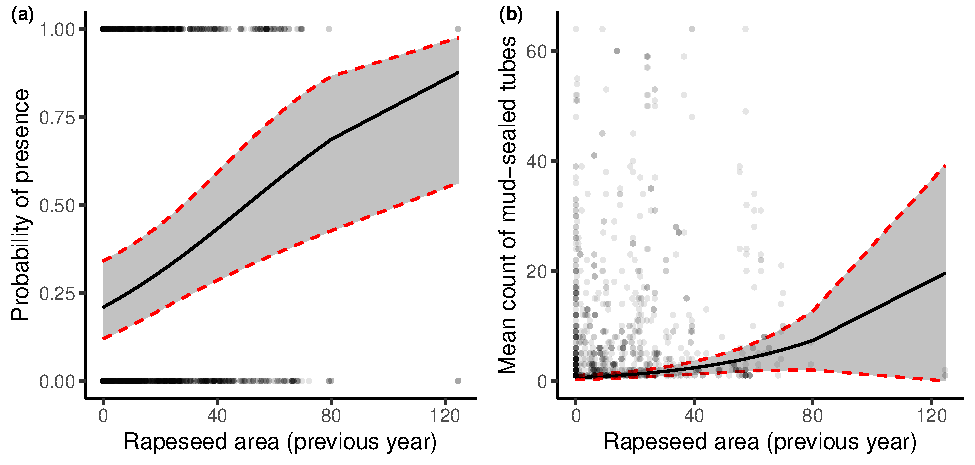
\includegraphics[width=1\linewidth]{solitary_bees_files/figure-latex/plots-rapeseed-1} \caption{Relationship between (\textbf{a}) probability of presence of a mud-sealed tube or (\textbf{b}) abundance of mud-sealed tubes, in trap nests set up in field crop edges, and rapeseed field area in the previous year. Line is (\textbf{a}) the predicted zero-inflation probability or (\textbf{b}) the mean model prediction conditioned on the fixed effects and the zero-inflation component. Ribbons are the confidence intervals.}\label{fig:plots-rapeseed}
\end{figure}

\begin{figure}
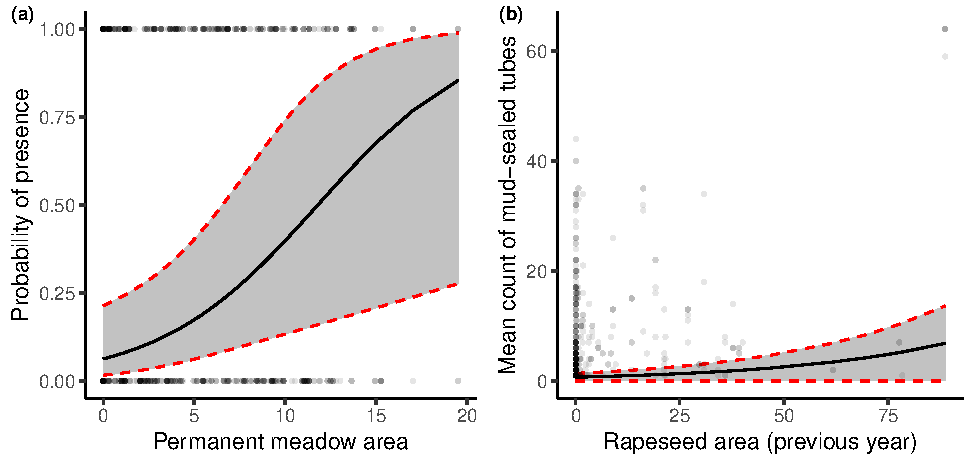
\includegraphics[width=1\linewidth]{solitary_bees_files/figure-latex/plots-meadowedge-1} \caption{Landscape covariates of the presence and abundance of mud-sealed tubes in trapnests set up in meadow edges. (\textbf{a}) Relationship between probability of presence of a mud-sealed tube and permanent meadow area. Line is the predicted zero-inflation probability. (\textbf{b}) Relationship between abundance of mud-sealed tubes and rapeseed field area in the previous year. Line is the mean model prediction, conditioned on the fixed effects and the zero-inflation component. Ribbons are the confidence intervals.}\label{fig:plots-meadowedge}
\end{figure}

\begin{figure}
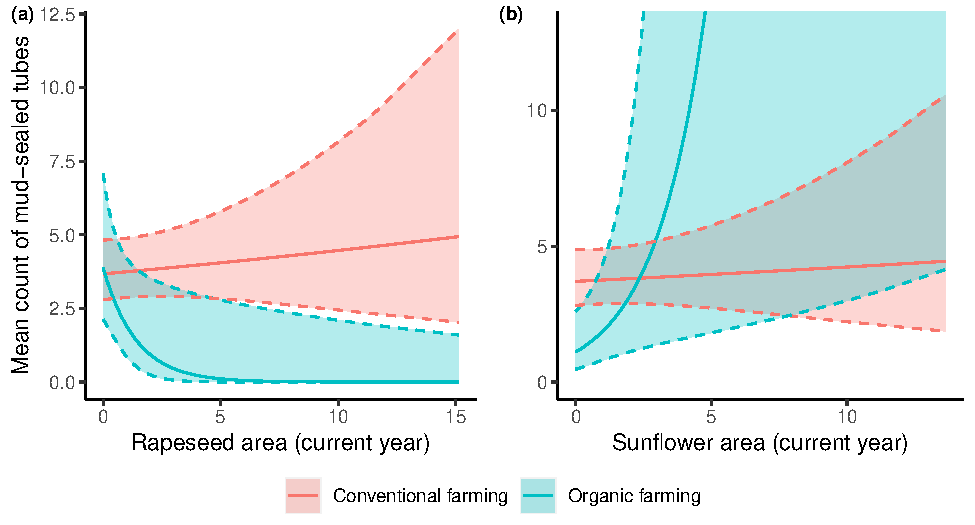
\includegraphics[width=1\linewidth]{solitary_bees_files/figure-latex/plots-interac-1} \caption{Relationship between abundance of mud-sealed tubes and mass-flowering crop area (\textbf{(a)} rapeseed,  or \textbf{(b)} sunflower), for trap nests set up in field crop edges across different farming systems. Lines are the mean model predictions, conditioned on the fixed effects and the zero-inflation component. Ribbons are the confidence intervals.}\label{fig:plots-interac}
\end{figure}

\begin{figure}
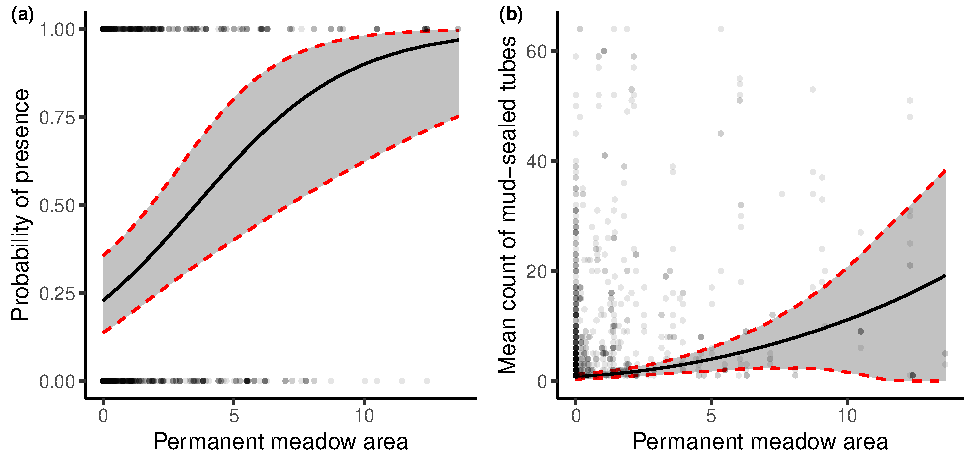
\includegraphics[width=1\linewidth]{solitary_bees_files/figure-latex/plots-meadow-1} \caption{Relationship between (\textbf{a}) probability of presence of a mud-sealed tube or (\textbf{b}) abundance of mud-sealed tubes, in trap nests set up in field crop edges, and permanent meadow area. Line is (\textbf{a}) the predicted zero-inflation probability or (\textbf{b}) the mean model prediction conditioned on the fixed effects and the zero-inflation component. Ribbons are the confidence intervals.}\label{fig:plots-meadow}
\end{figure}

\hypertarget{relationship-between-area-of-mass-flowering-crops-and-bee-reproduction}{%
\subsection{Relationship between area of mass-flowering crops and bee
reproduction}\label{relationship-between-area-of-mass-flowering-crops-and-bee-reproduction}}

Solitary bee reproduction was positively correlated with the quantity of
floral ressources provided by MFCs, only for rapeseed cultivated the
year preceding observations (Table \ref{tab:output}, \emph{area of
rapeseed (previous year)}). The area of rapeseed fields in the previous
year was positively linked to the presence and the abundance of
mud-sealed tubes in field crop edges (Fig. \ref{fig:plots-rapeseed}),
and only to the abundance of mud-sealed tubes in meadow edges (Fig.
\ref{fig:plots-meadowedge}b). In contrast, the area of rapeseed fields
in the current year did not correlate significantly with bee
reproduction, regardless of the model (Table \ref{tab:output},
\emph{area of rapeseed (current year)}). The area of sunflower fields in
the previous year was negatively linked to the presence of mud-sealed
tubes in field crop edges (Table \ref{tab:output}, \emph{area of
sunflower (previous year)}). In all other cases, there was no
significant correlation with bee reproduction.

In addition to the simple effect of previous year MFC area, we observed
significant interactions of current-year MFC area with the farming
system, although the latter did not have a significant simple effect
(Table \ref{tab:output}, \emph{area of rapeseed (cur. year):organic
farming} and \emph{area of sunflower (cur. year):organic farming}).
These interactions differed between MFCs. With rapeseed, the
relationship between mud-sealed tube abundance and coexisting crop area
varied from slightly positive to negative in conventional vs.~organic
fields (Fig. \ref{fig:plots-interac}a). In contrast, with sunflower, the
same relationship varied from slightly positive to strongly positive in
conventional vs.~organic fields (Fig. \ref{fig:plots-interac}b).

\hypertarget{relationship-between-landscape-elements-and-bee-reproduction}{%
\subsection{Relationship between landscape elements and bee
reproduction}\label{relationship-between-landscape-elements-and-bee-reproduction}}

The presence and abundance of mud-sealed tubes also correlated
significantly with the area of semi-natural elements likely to provide
food or nesting sources (Table \ref{tab:output}, \emph{area of permanent
meadows}). Both presence and abundance of mud-sealed tubes were
positively correlated with the area of permanent meadows in field crop
edge (Fig. \ref{fig:plots-meadow}). In meadow edge, the presence of
mud-sealed tubes, but not the abundance, was positively linked to
permanent meadow area (Fig. \ref{fig:plots-meadowedge}a). Temporary
meadows had more variable relationships with solitary bee reproduction.
In meadow edges, temporary meadow area in the current year was
positively related to solitary bee presence, but this area in the
previous year was negatively related to the presence of solitary bees
(Zero model in Table \ref{tab:output}, \emph{area of temporary
meadows}). The pattern was opposite for solitary bee abundance (Count
model in Table \ref{tab:output}, \emph{area of temporary meadows}). The
presence of mud-sealed tubes was positively related to perimeter of
forests in field crop edge, but the presence of hedgerows had no
detectable correlation in any model. The proximity of a road was
negatively related to the abundance of sealed tubes in meadow edges, and
to the presence of sealed tubes in field crop edges. Finally, the type
of the meadow was not significantly correlated with bee reproduction
measured in meadow edges.

\hypertarget{control-variables-1}{%
\subsection{Control variables}\label{control-variables-1}}

In all models, the number of days since the beginning of the year was
positively related to the presence of mud-sealed tubes. Similarly, when
significant, mean temperature and sum of precipitation correlated
positively with both presence and abundance of mud-sealed tubes.

\hypertarget{discussion}{%
\section{Discussion}\label{discussion}}

\hypertarget{inter-annual-impacts-of-mass-flowering-crops-on-solitary-bee-nest-building}{%
\subsection{Inter-annual impacts of mass flowering crops on solitary bee
nest
building}\label{inter-annual-impacts-of-mass-flowering-crops-on-solitary-bee-nest-building}}

We focused our study on the inter-annual effects of landscape floral
resources on the reproduction of one group of solitary bees (mostly
\emph{Osmia}). We evidenced a positive correlation between rapeseed
field area in the previous year and solitary bee nesting, both in the
zero model and the abundance model. Such correlation suggests that
rapeseed may have a lasting year-to-year impact on bee reproduction.
Whereas solitary bee nest-building was previously shown to increase
during the period of mass-flowering (Jauker, Peter, et al. 2012), we did
not find any significant impact of the area of rapeseed of the current
year. Our results indicate that the previous year resources seem to
benefit more to the nest-building and thus to support production of
sexuals, a requirement to carry over benefits into the next season.

Rapeseed floral ressources may promote a higher reproductive potential
the following year. Although both solitary bee males and females feed on
flowers, only females invest in brood care. During spring, solitary bee
females collect building materials and food for the nest, where the eggs
are lain in individual cells. The larvae stay in the nest throughout the
summer and winter, using pollen reserves, and emerge the following
spring. Reproductive success thus depends on the female's ability to
provision nests with enough pollen mixture to ensure the emergence of
enough offsprings the following year. Trap nests only provide
information about the number of sealed tubes, and not about the actual
number of cells and larvae in each tube. We do not know the actual
number of viable offsprings that will emerge the following spring: in
previous studies, it has been shown that sometimes no adults emerge from
a nest, notably because all cells can be parasitized (e.g.
Steffan-Dewenter 2002). This may explain why solitary bee reproduction
does not seem to depend on the area of rapeseed growing simultaneously:
available floral resources during breeding season allow each female to
lay more eggs in each tube (and to provision more pollen mixture for
each larvae) which will result in a higher abundance in the next year,
but not necessarily to seal more tubes because of the high cost of the
nest plug (Rust 1993). This explains why the effect of current rapeseed
cover is not significant. Riedinger et al. (2015) showed that rapeseed
has a year-to-year effect by promoting a higher solitary bee abundance
the following year. Here we show that this higher abundance of solitary
bees, which we did not measure directly, also translates into higher
reproductive potential, and indirect piece of evidence that rapeseed
promotes solitary bee population (Fig. \ref{fig:schema}). This result is
not obvious, since the rapeseed blooming period is limited, and since
its pollen may be of minor importance for larvae diet (Coudrain et al.
2016). Moreover, as a result of crop rotation, a high rapeseed cover one
year may lead to a lack of floral resources in the landscape the
following year.

\begin{figure}[]
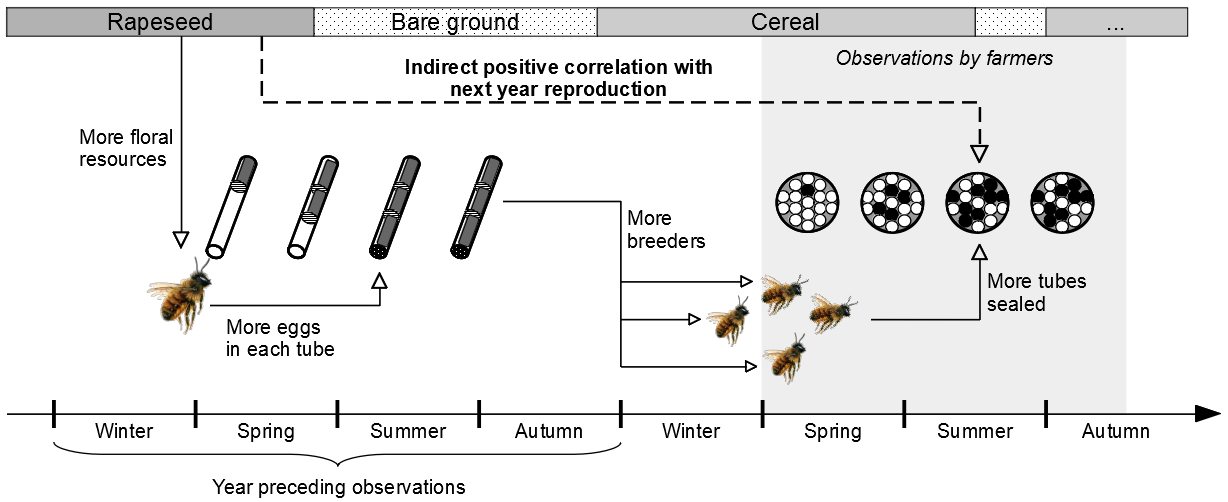
\includegraphics[width=1\linewidth]{solitary_bees_files/figure-latex/schema.png} \caption{Schematic summary of possible inter-annual effect of rapeseed floral resources on solitary bee reproduction. \emph{Osmia rufa} drawing by Valerie Littlewood, used with permission.}\label{fig:schema}
\end{figure}

Sunflower was differently correlated with bee reproduction. Unlike
rapeseed that blooms in spring, sunflower is a summer crop. The fact
that sunflower was not significantly related to bee reproduction in most
cases may confirm that mud-sealed tubes mainly concern solitary bees
active in early spring, such as \emph{Osmia}, which are known to
pollinate spring-blooming crops (Bosch, Sgolastra, and Kemp 2008).
Sunflower area was negatively correlated with bee reproduction the next
year only in the presence model, in field crop edges. This negative
correlation between sunflower field area in the previous year and the
presence of mud-sealed nests may be understood according to the same
logic of interpretation as the one adopted in the case of the effects of
rapeseed. Since sunflower is a summer crop sown in April, a high cover
leads to a lack of floral resources during the spring and may therefore
reduce the number of breeders in the next year. However, according to
this hypothesis, the abudance of mud-sealed tubes should also have been
negatively correlated to sunflower field area in the previous year, and
not only to the presence.~

We did not find any correlation with the area of MFC growing
simultaneously but the interactions between MFC cover in the current
year and farming system were significant, in a surprising way. We
expected local pesticide use intensity to have negative effects on bee
reproduction, and even to counteract the positive effects of MFC floral
resources and semi-natural habitats as demonstrated for pest biological
control (Ricci et al. 2019). Our analyses did not confirm these
predictions, since farming system alone did not have any significant
effect and conventional practices interacted positively with MFC
resources (Fig. \ref{fig:plots-interac}). We did not measure the number
of offsprings directly : pesticide exposure might not reduce nesting,
but only reduce offspring production and alter the sex-ratio (Stuligross
and Williams 2020). However, model outputs still confirm that local
practices should be taken into account when assessing the influence of
landscape context. Indeed, the landscape rapeseed area in the current
year correlated differently with the number of solitary bee nests
depending on local farming practices: no significant correlation under
conventional agricultural practices, but a negative correlation under
organic agricultural practices. These results can be interpreted
hypothetically as follows. A neighbouring field under organic farming
increases the number of weeds, which provide local floral resources
without pesticides for wild bees (Bretagnolle and Gaba 2015). This may
support a more diverse bee community (Carrié, Ekroos, and Smith 2018),
but perhaps with species that are less tolerant to pesticides used in
the surrounding rapeseed fields (B. A. Woodcock et al. 2017). Thus, a
higher rapeseed cover in the landscape could have a negative impact on
the bees present in the edge of an organic field. On the contrary, wild
bees in the edge of a conventional field may be less diversified but
more tolerant to pesticides. However, we did not study the whole wild
bee community, but only solitary bees related to mud-sealed tubes (a
majority of \emph{Osmia}), which reduces the likelihood that
closely-related species express different tolerance to pesticides. In
addition, we had information on the farming system only for the field in
which the trap nests were placed, which seriously limits our ability to
interpret any interaction between the effects of MFC area at the
landscape scale and farming practices on solitary bee reproduction.

\hypertarget{importance-of-semi-natural-elements-and-other-permanent-landscape-features}{%
\subsection{Importance of semi-natural elements and other permanent
landscape
features}\label{importance-of-semi-natural-elements-and-other-permanent-landscape-features}}

Both for the probability of presence and abundance of sealed tubes, the
area of permanent meadows in the buffer strongly promoted solitary bee
reproduction. This is consistent with previous studies which showed that
loss of semi-natural habitats, i.e.~land uses that are minimally managed
and not cultivated for arable crops, is one of the main drivers of
pollinator decline (Ricketts et al. 2008; Tscharntke et al. 2012). As
the dynamics of bee populations are mainly driven by the amount of
nesting and floral resources (Lonsdorf et al. 2009), semi-natural areas
help maintain bee populations (Carré et al. 2009; Tscharntke et al.
2012) by providing both nesting and food opportunities. Remaining
permanent meadows may also be important to offset bee decline caused by
meadow-to-crop conversion that occurred long ago (Provost et al. 2020).
Moreover, these semi-natural habitats may decrease the negative effect
of warmer temperature on bee populations (Papanikolaou et al. 2017) and
buffer the harmful impacts of pesticides (Park et al. 2015).

In both our models however, there was no evidence of a positive effect
of the proximity of hedgerows. This is against our expectations, since
it has been shown that abundance and diversity of wild bees are enhanced
in field edges by hedgerows (Morandin and Kremen 2013). This result may
be due to the fact that this parameter is reported by farmers, whose
definition of a hedgerow may differ and may include different types of
vegetation and different stages of the hedgerows (recently planted or
older, more or less diversified). By contrast, our models evidenced a
negative impact of the presence of a road. The amount of roads has
already been shown to decrease bumblebee density (Kallioniemi et al.
2017), but road verges could also provide floral resources for wild bees
(Henriksen and Langer 2013).

Semi-natural areas and mass-flowering crops do not have the same
relative importance. In both zero models, the area of permanent meadows
had a stronger positive effect than the area of rapeseed in the previous
year. On the contrary, in both count models, the impact of rapeseed was
slightly to really stronger. The presence of solitary bees seems to
depend more on the semi-natural areas while their abundance seems to
depend more on the ressources provided by rapeseed. Nevertheless, the
permanent meadow area does not condition the positive effect of
rapeseed: we tested the interaction between the two variables and we did
not find any significant correlation (not shown). The presence of
permenant meadows may be a important factor when a solitary bee chooses
where to build its nest, because some wild flowers in meadows are in
bloom before rapeseed fields and thus are more attractive. Once the nest
is built, rapeseed will provide a massive amount of pollen and nectar to
solitary bees active during its flowering period (such as \emph{Osmia}),
allowing each female to lay more eggs in each tube and thus increasing
the number of breeders the following year.

\hypertarget{conclusion-implications-for-pollinator-conservation-in-agricultural-landscapes}{%
\section{Conclusion: implications for pollinator conservation in
agricultural
landscapes}\label{conclusion-implications-for-pollinator-conservation-in-agricultural-landscapes}}

Defining how agriculturally dominated landscape can be optimized for
wild bees remains a complex subject. Our study shows that solitary bee
reproduction can be positively and durably affected by rapeseed cover.
This crop provides a massive amount of floral resources at a period
favorable for wild bees such as \emph{Osmia}. Moreover, our study
confirms that permanent meadows are essential to promote solitary bee
populations. The positive effect of rapeseed cover may hold only if
enough food and nesting sites are available in adjacent natural
habitats. Ricketts et al. (2008) showed that flower‐visitor richness and
visitation rate in croplands decline with distance from natural areas,
and a lack of natural habitats can directly impact on crop yield (Lucas
A. Garibaldi et al. 2011; Holzschuh et al. 2012). Protecting natural
habitats near crop fields seems to be a key solution to secure natural
supply of pollination service, and moderate covers of rapeseed may help
to maintain solitary bee populations. However, rapeseed flowering period
is short, thus pollinators still need floral resources from other crops
and other semi-natural habitats (Martins et al. 2018), especially as we
studied a small part of the wild bee community. The use of rapeseed for
promoting wild pollinators needs also to be viewed bearing in mind the
heavy pesticide application on this crop.

(MacIvor and Packer 2015)

\hypertarget{references}{%
\section{References}\label{references}}

\hypertarget{refs}{}
\begin{CSLReferences}{1}{0}
\leavevmode\vadjust pre{\hypertarget{ref-artz2015}{}}%
Artz, Derek R., and Theresa L. Pitts-Singer. 2015. {``Effects of
Fungicide and Adjuvant Sprays on Nesting Behavior in Two Managed
Solitary Bees, \emph{{O}smia Lignaria} and \emph{{M}egachile
Rotundata}.''} Edited by Nicolas Desneux. \emph{{PLOS} {ONE}} 10 (8):
e0135688. \url{https://doi.org/10.1371/journal.pone.0135688}.

\leavevmode\vadjust pre{\hypertarget{ref-azpiazu2019}{}}%
Azpiazu, Celeste, Jordi Bosch, Elisa Viñuela, Piotr Medrzycki, Dariusz
Teper, and Fabio Sgolastra. 2019. {``Chronic Oral Exposure to
Field-Realistic Pesticide Combinations via Pollen and Nectar: Effects on
Feeding and Thermal Performance in a Solitary Bee.''} \emph{Scientific
Reports} 9 (1). \url{https://doi.org/10.1038/s41598-019-50255-4}.

\leavevmode\vadjust pre{\hypertarget{ref-bailey2014}{}}%
Bailey, Samantha, Fabrice Requier, Benoit Nusillard, Stuart P. M.
Roberts, Simon G. Potts, and Christophe Bouget. 2014. {``Distance from
Forest Edge Affects Bee Pollinators in Oilseed Rape Fields.''}
\emph{Ecology and Evolution} 4 (4): 370--80.
\url{https://doi.org/10.1002/ece3.924}.

\leavevmode\vadjust pre{\hypertarget{ref-barton2020}{}}%
Bartoń, Kamil. 2020. \emph{MuMIn: Multi-Model Inference}.
\url{https://CRAN.R-project.org/package=MuMIn}.

\leavevmode\vadjust pre{\hypertarget{ref-benton2002}{}}%
Benton, Tim G., David M. Bryant, Lorna Cole, and Humphrey Q. P. Crick.
2002. {``Linking Agricultural Practice to Insect and Bird Populations: A
Historical Study over Three Decades.''} \emph{Journal of Applied
Ecology} 39 (4): 673--87.
\url{https://doi.org/10.1046/j.1365-2664.2002.00745.x}.

\leavevmode\vadjust pre{\hypertarget{ref-biddinger2013}{}}%
Biddinger, Jacqueline L. AND Mullin, David J. AND Robertson. 2013.
{``Comparative Toxicities and Synergism of Apple Orchard Pesticides to
\emph{{A}pis Mellifera} ({L}.) And \emph{{O}smia Cornifrons}
({R}adoszkowski).''} \emph{PLOS ONE} 8 (9): 1--6.
\url{https://doi.org/10.1371/journal.pone.0072587}.

\leavevmode\vadjust pre{\hypertarget{ref-biesmeijer2006}{}}%
Biesmeijer, J. C., S. P. M. Roberts, M. Reemer, R. Ohlemüller, M.
Edwards, T. Peeters, A. P. Schaffers, et al. 2006. {``Parallel Declines
in Pollinators and Insect-Pollinated Plants in {B}ritain and the
{N}etherlands.''} \emph{Science} 313 (5785): 351--54.
\url{https://doi.org/10.1126/science.1127863}.

\leavevmode\vadjust pre{\hypertarget{ref-billaud2020}{}}%
Billaud, Olivier, Rose-Line Vermeersch, and Emmanuelle Porcher. 2020.
{``Citizen Science Involving Farmers as a Means to Document Temporal
Trends in Farmland Biodiversity and Relate Them to Agricultural
Practices.''} \emph{Journal of Applied Ecology}.
\url{https://doi.org/10.1111/1365-2664.13746}.

\leavevmode\vadjust pre{\hypertarget{ref-bosch2008}{}}%
Bosch, Jordi, Fabio Sgolastra, and William P. Kemp. 2008. {``6. Life
Cycle Ecophysiology of Osmia Mason Bees Used as Crop Pollinators.''} In
\emph{Bee Pollination in Agricultural Eco-Systems}, 83--105. Oxford
University Press.
\url{https://doi.org/10.1093/acprof:oso/9780195316957.003.0006}.

\leavevmode\vadjust pre{\hypertarget{ref-bretagnolle2015}{}}%
Bretagnolle, Vincent, and Sabrina Gaba. 2015. {``Weeds for Bees? A
Review.''} \emph{Agronomy for Sustainable Development} 35 (3): 891--909.
\url{https://doi.org/10.1007/s13593-015-0302-5}.

\leavevmode\vadjust pre{\hypertarget{ref-mollie2017}{}}%
Brooks, Mollie E., Kasper Kristensen, Koen J. van Benthem, Arni
Magnusson, Casper W. Berg, Anders Nielsen, Hans J. Skaug, Martin
Maechler, and Benjamin M. Bolker. 2017. {``{glmmTMB} Balances Speed and
Flexibility Among Packages for Zero-Inflated Generalized Linear Mixed
Modeling.''} \emph{The R Journal} 9 (2): 378--400.
\url{https://journal.r-project.org/archive/2017/RJ-2017-066/index.html}.

\leavevmode\vadjust pre{\hypertarget{ref-burkle2013}{}}%
Burkle, Laura A., John C. Marlin, and Tiffany M. Knight. 2013.
{``Plant-Pollinator Interactions over 120 Years: Loss of Species,
Co-Occurrence, and Function.''} \emph{Science} 339 (6127): 1611--15.
\url{https://doi.org/10.1126/science.1232728}.

\leavevmode\vadjust pre{\hypertarget{ref-carre2009}{}}%
Carré, Gabriel, Philip Roche, Rémy Chifflet, Nicolas Morison, Riccardo
Bommarco, Jenn Harrison-Cripps, Kristin Krewenka, et al. 2009.
{``Landscape Context and Habitat Type as Drivers of Bee Diversity in
European Annual Crops.''} \emph{Agriculture, Ecosystems and Environment}
133 (1): 40--47.
https://doi.org/\url{https://doi.org/10.1016/j.agee.2009.05.001}.

\leavevmode\vadjust pre{\hypertarget{ref-carrie2018}{}}%
Carrié, Romain, Johan Ekroos, and Henrik G. Smith. 2018. {``Organic
Farming Supports Spatiotemporal Stability in Species Richness of
Bumblebees and Butterflies.''} \emph{Biological Conservation} 227:
48--55.
https://doi.org/\url{https://doi.org/10.1016/j.biocon.2018.08.022}.

\leavevmode\vadjust pre{\hypertarget{ref-cornes2018}{}}%
Cornes, Richard C., Gerard van der Schrier, Else J. M. van den
Besselaar, and Philip D. Jones. 2018. {``An Ensemble Version of the
e-OBS Temperature and Precipitation Data Sets.''} \emph{Journal of
Geophysical Research: Atmospheres} 123 (17): 9391--9409.
\url{https://doi.org/10.1029/2017JD028200}.

\leavevmode\vadjust pre{\hypertarget{ref-coudrain2016}{}}%
Coudrain, Valérie, Sarah Rittiner, Felix Herzog, Willy Tinner, and
Martin H. Entling. 2016. {``Landscape Distribution of Food and Nesting
Sites Affect Larval Diet and Nest Size, but Not Abundance of Osmia
Bicornis.''} \emph{Insect Science} 23 (5): 746--53.
\url{https://doi.org/10.1111/1744-7917.12238}.

\leavevmode\vadjust pre{\hypertarget{ref-diekotter2010}{}}%
Diekötter, Tim, Taku Kadoya, Franziska Peter, Volkmar Wolters, and Frank
Jauker. 2010. {``Oilseed Rape Crops Distort Plant--Pollinator
Interactions.''} \emph{Journal of Applied Ecology} 47 (1): 209--14.
https://doi.org/\url{https://doi.org/10.1111/j.1365-2664.2009.01759.x}.

\leavevmode\vadjust pre{\hypertarget{ref-diekotter2014}{}}%
Diekötter, Tim, Franziska Peter, Birgit Jauker, Volkmar Wolters, and
Frank Jauker. 2014. {``Mass-Flowering Crops Increase Richness of
Cavity-Nesting Bees and Wasps in Modern Agro-Ecosystems.''} \emph{GCB
Bioenergy} 6 (3): 219--26. \url{https://doi.org/10.1111/gcbb.12080}.

\leavevmode\vadjust pre{\hypertarget{ref-garibaldi2011}{}}%
Garibaldi, Lucas A., Ingolf Steffan-Dewenter, Claire Kremen, Juan M.
Morales, Riccardo Bommarco, Saul A. Cunningham, Luísa G. Carvalheiro, et
al. 2011. {``Stability of Pollination Services Decreases with Isolation
from Natural Areas Despite Honey Bee Visits.''} \emph{Ecology Letters}
14 (10): 1062--72.
\url{https://doi.org/10.1111/j.1461-0248.2011.01669.x}.

\leavevmode\vadjust pre{\hypertarget{ref-garibaldi2014}{}}%
Garibaldi, Lucas A, Luísa G Carvalheiro, Sara D Leonhardt, Marcelo A
Aizen, Brett R Blaauw, Rufus Isaacs, Michael Kuhlmann, et al. 2014.
{``From Research to Action: Enhancing Crop Yield Through Wild
Pollinators.''} \emph{Frontiers in Ecology and the Environment} 12 (8):
439--47. \url{https://doi.org/10.1890/130330}.

\leavevmode\vadjust pre{\hypertarget{ref-goulson2008}{}}%
Goulson, D., G. C. Lye, and B. Darvill. 2008. {``Decline and
Conservation of Bumble Bees.''} \emph{Annual Review of Entomology} 53
(1): 191--208.
\url{https://doi.org/10.1146/annurev.ento.53.103106.093454}.

\leavevmode\vadjust pre{\hypertarget{ref-dharma2020}{}}%
Hartig, Florian. 2020. \emph{DHARMa: Residual Diagnostics for
Hierarchical (Multi-Level / Mixed) Regression Models}.
\url{https://CRAN.R-project.org/package=DHARMa}.

\leavevmode\vadjust pre{\hypertarget{ref-henriksen2013}{}}%
Henriksen, Casper Ingerslev, and Vibeke Langer. 2013. {``Road Verges and
Winter Wheat Fields as Resources for Wild Bees in Agricultural
Landscapes.''} \emph{Agriculture, Ecosystems \& Environment} 173:
66--71.
https://doi.org/\url{https://doi.org/10.1016/j.agee.2013.04.008}.

\leavevmode\vadjust pre{\hypertarget{ref-holzschuh2016}{}}%
Holzschuh, Andrea, Matteo Dainese, Juan P. González-Varo, Sonja
Mudri-Stojnić, Verena Riedinger, Maj Rundlöf, Jeroen Scheper, et al.
2016. {``Mass-Flowering Crops Dilute Pollinator Abundance in
Agricultural Landscapes Across Europe.''} \emph{Ecology Letters} 19
(10): 1228--36. \url{https://doi.org/10.1111/ele.12657}.

\leavevmode\vadjust pre{\hypertarget{ref-holzschuh2012}{}}%
Holzschuh, Andrea, Carsten F. Dormann, Teja Tscharntke, and Ingolf
Steffan-Dewenter. 2012. {``Mass-Flowering Crops Enhance Wild Bee
Abundance.''} \emph{Oecologia} 172 (2): 477--84.
\url{https://doi.org/10.1007/s00442-012-2515-5}.

\leavevmode\vadjust pre{\hypertarget{ref-jackson2015}{}}%
Jackson, Heather Bird, and Lenore Fahrig. 2015. {``Are Ecologists
Conducting Research at the Optimal Scale?''} \emph{Global Ecology and
Biogeography} 24 (1): 52--63. \url{https://doi.org/10.1111/geb.12233}.

\leavevmode\vadjust pre{\hypertarget{ref-jauker2012a}{}}%
Jauker, Frank, Birgit Bondarenko, Heiko C. Becker, and Ingolf
Steffan-Dewenter. 2012. {``Pollination Efficiency of Wild Bees and
Hoverflies Provided to Oilseed Rape.''} \emph{Agricultural and Forest
Entomology} 14 (1): 81--87.
\url{https://doi.org/10.1111/j.1461-9563.2011.00541.x}.

\leavevmode\vadjust pre{\hypertarget{ref-jauker2012b}{}}%
Jauker, Frank, Franziska Peter, Volkmar Wolters, and Tim Diekötter.
2012. {``Early Reproductive Benefits of Mass-Flowering Crops to the
Solitary Bee \emph{{O}smia Rufa} Outbalance Post-Flowering
Disadvantages.''} \emph{Basic and Applied Ecology} 13 (3): 268--76.
https://doi.org/\url{https://doi.org/10.1016/j.baae.2012.03.010}.

\leavevmode\vadjust pre{\hypertarget{ref-joshi2016}{}}%
Joshi, Neelendra K., Mark Otieno, Edwin G. Rajotte, Shelby J. Fleischer,
and David J. Biddinger. 2016. {``Proximity to Woodland and Landscape
Structure Drives Pollinator Visitation in Apple Orchard Ecosystem.''}
\emph{Frontiers in Ecology and Evolution} 4: 38.
\url{https://doi.org/10.3389/fevo.2016.00038}.

\leavevmode\vadjust pre{\hypertarget{ref-kallioniemi2017}{}}%
Kallioniemi, Eveliina, Jens Åström, Graciela M. Rusch, Sondre Dahle,
Sandra Åström, and Jan Ove Gjershaug. 2017. {``Local Resources, Linear
Elements and Mass-Flowering Crops Determine Bumblebee Occurrences in
Moderately Intensified Farmlands.''} \emph{Agriculture, Ecosystems \&
Environment} 239: 90--100.
https://doi.org/\url{https://doi.org/10.1016/j.agee.2016.12.039}.

\leavevmode\vadjust pre{\hypertarget{ref-klein2007}{}}%
Klein, Alexandra-Maria, Bernard E Vaissière, James H Cane, Ingolf
Steffan-Dewenter, Saul A Cunningham, Claire Kremen, and Teja Tscharntke.
2007. {``Importance of Pollinators in Changing Landscapes for World
Crops.''} \emph{Proceedings of the Royal Society B: Biological Sciences}
274 (1608): 303--13. \url{https://doi.org/10.1098/rspb.2006.3721}.

\leavevmode\vadjust pre{\hypertarget{ref-lefeon2013}{}}%
Le Féon, Violette, Françoise Burel, Rémy Chifflet, Mickaël Henry, Agnès
Ricroch, Bernard E. Vaissière, and Jacques Baudry. 2013. {``Solitary Bee
Abundance and Species Richness in Dynamic Agricultural Landscapes.''}
\emph{Agriculture, Ecosystems and Environment} 166: 94--101.
https://doi.org/\url{https://doi.org/10.1016/j.agee.2011.06.020}.

\leavevmode\vadjust pre{\hypertarget{ref-leifeld2013}{}}%
Leifeld, Philip. 2013. {``{texreg}: Conversion of Statistical Model
Output in {R} to {LaTeX} and {HTML} Tables.''} \emph{Journal of
Statistical Software} 55 (8): 1--24.
\url{http://www.jstatsoft.org/v55/i08/}.

\leavevmode\vadjust pre{\hypertarget{ref-linsley1958}{}}%
Linsley, E. Gorton. 1958. {``The Ecology of Solitary Bees.''}
\emph{Hilgardia} 27 (19): 543--99.
\url{https://doi.org/10.3733/hilg.v27n19p543}.

\leavevmode\vadjust pre{\hypertarget{ref-lonsdorf2009}{}}%
Lonsdorf, Eric, Claire Kremen, Taylor Ricketts, Rachael Winfree, Neal
Williams, and Sarah Greenleaf. 2009. {``{Modelling pollination services
across agricultural landscapes}.''} \emph{Annals of Botany} 103 (9):
1589--1600. \url{https://doi.org/10.1093/aob/mcp069}.

\leavevmode\vadjust pre{\hypertarget{ref-ludecke2018}{}}%
Lüdecke, Daniel. 2018. {``Ggeffects: Tidy Data Frames of Marginal
Effects from Regression Models.''} \emph{Journal of Open Source
Software} 3 (26): 772. \url{https://doi.org/10.21105/joss.00772}.

\leavevmode\vadjust pre{\hypertarget{ref-ludecke2020}{}}%
Lüdecke, Daniel, Dominique Makowski, Philip Waggoner, and Indrajeet
Patil. 2020. \emph{Performance: Assessment of Regression Models
Performance}. \url{https://CRAN.R-project.org/package=performance}.

\leavevmode\vadjust pre{\hypertarget{ref-macivor2015}{}}%
MacIvor, J. Scott, and Laurence Packer. 2015. {``{`Bee Hotels'} as Tools
for Native Pollinator Conservation: A Premature Verdict?''} Edited by
Fabio S. Nascimento. \emph{{PLOS} {ONE}} 10 (3): e0122126.
\url{https://doi.org/10.1371/journal.pone.0122126}.

\leavevmode\vadjust pre{\hypertarget{ref-mallinger2014}{}}%
Mallinger, Rachel E., and Claudio Gratton. 2015. {``Species Richness of
Wild Bees, but Not the Use of Managed Honeybees, Increases Fruit Set of
a Pollinator-Dependent Crop.''} \emph{Journal of Applied Ecology} 52
(2): 323--30. \url{https://doi.org/10.1111/1365-2664.12377}.

\leavevmode\vadjust pre{\hypertarget{ref-martins2018}{}}%
Martins, Kyle T., Cécile H. Albert, Martin J. Lechowicz, and Andrew
Gonzalez. 2018. {``Complementary Crops and Landscape Features Sustain
Wild Bee Communities.''} \emph{Ecological Applications} 28 (4):
1093--1105. \url{https://doi.org/10.1002/eap.1713}.

\leavevmode\vadjust pre{\hypertarget{ref-michener2007}{}}%
Michener, Charles. 2007. \emph{The Bees of the World}. Baltimore: Johns
Hopkins University Press.
\url{https://jhupbooks.press.jhu.edu/title/bees-world}.

\leavevmode\vadjust pre{\hypertarget{ref-morandin2013}{}}%
Morandin, Lora A., and Claire Kremen. 2013. {``Hedgerow Restoration
Promotes Pollinator Populations and Exports Native Bees to Adjacent
Fields.''} \emph{Ecological Applications} 23 (4): 829--39.
\url{https://doi.org/10.1890/12-1051.1}.

\leavevmode\vadjust pre{\hypertarget{ref-odanaka2020}{}}%
Odanaka, Katherine A., and Sandra M. Rehan. 2020. {``Wild Bee
Distribution Near Forested Landscapes Is Dependent on Successional
State.''} \emph{Forest Ecosystems} 7 (1).
\url{https://doi.org/10.1186/s40663-020-00241-4}.

\leavevmode\vadjust pre{\hypertarget{ref-ollerton2011}{}}%
Ollerton, Jeff, Rachael Winfree, and Sam Tarrant. 2011. {``How Many
Flowering Plants Are Pollinated by Animals?''} \emph{Oikos} 120 (3):
321--26. \url{https://doi.org/10.1111/j.1600-0706.2010.18644.x}.

\leavevmode\vadjust pre{\hypertarget{ref-papanikolaou2017}{}}%
Papanikolaou, Alexandra D., Ingolf Kühn, Mark Frenzel, and Oliver
Schweiger. 2017. {``Semi-Natural Habitats Mitigate the Effects of
Temperature Rise on Wild Bees.''} \emph{Journal of Applied Ecology} 54
(2): 527--36. \url{https://doi.org/10.1111/1365-2664.12763}.

\leavevmode\vadjust pre{\hypertarget{ref-park2015}{}}%
Park, Mia G., E. J. Blitzer, Jason Gibbs, John E. Losey, and Bryan N.
Danforth. 2015. {``Negative Effects of Pesticides on Wild Bee
Communities Can Be Buffered by Landscape Context.''} \emph{Proceedings
of the Royal Society B: Biological Sciences} 282 (1809): 20150299.
\url{https://doi.org/10.1098/rspb.2015.0299}.

\leavevmode\vadjust pre{\hypertarget{ref-edzer2018}{}}%
Pebesma, Edzer. 2018. {``{Simple Features for R: Standardized Support
for Spatial Vector Data}.''} \emph{{The R Journal}} 10 (1): 439--46.
\url{https://doi.org/10.32614/RJ-2018-009}.

\leavevmode\vadjust pre{\hypertarget{ref-peixoto2014}{}}%
Pereira-Peixoto, Maria Helena, Gesine Pufal, Celso Feitosa Martins, and
Alexandra-Maria Klein. 2014. {``Spillover of Trap-Nesting Bees and Wasps
in an Urban{\textendash}rural Interface.''} \emph{Journal of Insect
Conservation} 18 (5): 815--26.
\url{https://doi.org/10.1007/s10841-014-9688-7}.

\leavevmode\vadjust pre{\hypertarget{ref-potts2006}{}}%
Potts, Joanne M., and Jane Elith. 2006. {``Comparing Species Abundance
Models.''} \emph{Ecological Modelling} 199 (2): 153--63.
https://doi.org/\url{https://doi.org/10.1016/j.ecolmodel.2006.05.025}.

\leavevmode\vadjust pre{\hypertarget{ref-potts2010}{}}%
Potts, Simon G., Jacobus C. Biesmeijer, Claire Kremen, Peter Neumann,
Oliver Schweiger, and William E. Kunin. 2010. {``Global Pollinator
Declines: Trends, Impacts and Drivers.''} \emph{Trends in Ecology and
Evolution} 25 (6): 345--53.
https://doi.org/\url{https://doi.org/10.1016/j.tree.2010.01.007}.

\leavevmode\vadjust pre{\hypertarget{ref-potts2003}{}}%
Potts, Simon G., Betsy Vulliamy, Amots Dafni, Gidi Ne'eman, and Pat
Willmer. 2003. {``Linking Bees and Flowers: How Do Floral Communities
Structure Pollinatore Communities?''} \emph{Ecology} 84 (10): 2628--42.
\url{https://doi.org/10.1890/02-0136}.

\leavevmode\vadjust pre{\hypertarget{ref-leprovost2020}{}}%
Provost, Gaëtane Le, Isabelle Badenhausser, Cyrille Violle, Fabrice
Requier, Marie D'Ottavio, Marilyn Roncoroni, Louis Gross, and Nicolas
Gross. 2020. {``Grassland-to-Crop Conversion in Agricultural Landscapes
Has Lasting Impact on the Trait Diversity of Bees.''} \emph{Landscape
Ecology}, October. \url{https://doi.org/10.1007/s10980-020-01141-2}.

\leavevmode\vadjust pre{\hypertarget{ref-rcore2020}{}}%
R Core Team. 2020. \emph{R: A Language and Environment for Statistical
Computing}. Vienna, Austria: R Foundation for Statistical Computing.
\url{https://www.R-project.org/}.

\leavevmode\vadjust pre{\hypertarget{ref-ricci2019}{}}%
Ricci, B., C. Lavigne, A. Alignier, S. Aviron, L. Biju-Duval, J. C.
Bouvier, J.-P. Choisis, et al. 2019. {``Local Pesticide Use Intensity
Conditions Landscape Effects on Biological Pest Control.''}
\emph{Proceedings of the Royal Society B: Biological Sciences} 286
(1904): 20182898. \url{https://doi.org/10.1098/rspb.2018.2898}.

\leavevmode\vadjust pre{\hypertarget{ref-ricketts2008}{}}%
Ricketts, Taylor H., James Regetz, Ingolf Steffan-Dewenter, Saul A.
Cunningham, Claire Kremen, Anne Bogdanski, Barbara Gemmill-Herren, et
al. 2008. {``Landscape Effects on Crop Pollination Services: Are There
General Patterns?''} \emph{Ecology Letters} 11 (5): 499--515.
\url{https://doi.org/10.1111/j.1461-0248.2008.01157.x}.

\leavevmode\vadjust pre{\hypertarget{ref-riedinger2015}{}}%
Riedinger, Verena, Oliver Mitesser, Thomas Hovestadt, Ingolf
Steffan-Dewenter, and Andrea Holzschuh. 2015. {``Annual Dynamics of Wild
Bee Densities: Attractiveness and Productivity Effects of Oilseed
Rape.''} \emph{Ecology} 96 (5): 1351--60.
\url{https://doi.org/10.1890/14-1124.1}.

\leavevmode\vadjust pre{\hypertarget{ref-rollin2013}{}}%
Rollin, Orianne, Vincent Bretagnolle, Axel Decourtye, Jean Aptel, Nadia
Michel, Bernard E. Vaissière, and Mickaël Henry. 2013. {``Differences of
Floral Resource Use Between Honey Bees and Wild Bees in an Intensive
Farming System.''} \emph{Agriculture, Ecosystems and Environment} 179:
78--86.
https://doi.org/\url{https://doi.org/10.1016/j.agee.2013.07.007}.

\leavevmode\vadjust pre{\hypertarget{ref-rstudio2019}{}}%
RStudio Team. 2019. \emph{RStudio: Integrated Development Environment
for r}. Boston, MA: RStudio, Inc. \url{http://www.rstudio.com/}.

\leavevmode\vadjust pre{\hypertarget{ref-rundlof2015}{}}%
Rundlöf, Maj, Georg K. S. Andersson, Riccardo Bommarco, Ingemar Fries,
Veronica Hederström, Lina Herbertsson, Ove Jonsson, et al. 2015. {``Seed
Coating with a Neonicotinoid Insecticide Negatively Affects Wild
Bees.''} \emph{Nature} 521 (7550): 77--80.
\url{https://doi.org/10.1038/nature14420}.

\leavevmode\vadjust pre{\hypertarget{ref-rust1993}{}}%
Rust, Richard W. 1993. {``{Cell and Nest Construction Costs in Two
Cavity-Nesting Bees (Osmia lignaria propinqua and Osmia ribifloris
biedermannii) (Hymenoptera: Megachilidae)}.''} \emph{Annals of the
Entomological Society of America} 86 (3): 327--32.
\url{https://doi.org/10.1093/aesa/86.3.327}.

\leavevmode\vadjust pre{\hypertarget{ref-sanchez2019}{}}%
Sánchez-Bayo, Francisco, and Kris A. G. Wyckhuys. 2019. {``Worldwide
Decline of the Entomofauna: A Review of Its Drivers.''} \emph{Biological
Conservation} 232: 8--27.
https://doi.org/\url{https://doi.org/10.1016/j.biocon.2019.01.020}.

\leavevmode\vadjust pre{\hypertarget{ref-sgolastra2017}{}}%
Sgolastra, Fabio, Piotr Medrzycki, Laura Bortolotti, Maria Teresa Renzi,
Simone Tosi, Gherardo Bogo, Dariusz Teper, Claudio Porrini, Roberto
Molowny-Horas, and Jordi Bosch. 2017. {``Synergistic Mortality Between a
Neonicotinoid Insecticide and an Ergosterol-Biosynthesis-Inhibiting
Fungicide in Three Bee Species.''} \emph{Pest Management Science} 73
(6): 1236--43. \url{https://doi.org/10.1002/ps.4449}.

\leavevmode\vadjust pre{\hypertarget{ref-shaw2020}{}}%
Shaw, Rosalind F., Benjamin B. Phillips, Toby Doyle, Judith K. Pell,
John W. Redhead, Joanna Savage, Ben A. Woodcock, James M. Bullock, and
Juliet L. Osborne. 2020. {``Mass-Flowering Crops Have a Greater Impact
Than Semi-Natural Habitat on Crop Pollinators and Pollen Deposition.''}
\emph{Landscape Ecology} 35 (2): 513--27.
\url{https://doi.org/10.1007/s10980-019-00962-0}.

\leavevmode\vadjust pre{\hypertarget{ref-steffandewenter2002}{}}%
Steffan-Dewenter, Ingolf. 2002. {``Landscape Context Affects
Trap-Nesting Bees, Wasps, and Their Natural Enemies.''} \emph{Ecological
Entomology} 27 (5): 631--37.
\url{https://doi.org/10.1046/j.1365-2311.2002.00437.x}.

\leavevmode\vadjust pre{\hypertarget{ref-dewenter2003}{}}%
Steffan-Dewenter, Ingolf, and Kathleen Leschke. 2003. {``Effects of
Habitat Management on Vegetation and Above-Ground Nesting Bees and Wasps
of Orchard Meadows in Central Europe.''} \emph{Biodiversity and
Conservation} 12 (9): 1953--68.
\url{https://doi.org/10.1023/a:1024199513365}.

\leavevmode\vadjust pre{\hypertarget{ref-stuligross2020}{}}%
Stuligross, Clara, and Neal M. Williams. 2020. {``Pesticide and Resource
Stressors Additively Impair Wild Bee Reproduction.''} \emph{Proceedings
of the Royal Society B: Biological Sciences} 287 (1935): 20201390.
\url{https://doi.org/10.1098/rspb.2020.1390}.

\leavevmode\vadjust pre{\hypertarget{ref-tscharntke2012}{}}%
Tscharntke, Teja, Jason M. Tylianakis, Tatyana A. Rand, Raphael K.
Didham, Lenore Fahrig, Péter Batáry, Janne Bengtsson, et al. 2012.
{``Landscape Moderation of Biodiversity Patterns and Processes - Eight
Hypotheses.''} \emph{Biological Reviews} 87 (3): 661--85.
\url{https://doi.org/10.1111/j.1469-185X.2011.00216.x}.

\leavevmode\vadjust pre{\hypertarget{ref-vanbergen2013}{}}%
Vanbergen, Adam J, and the Insect Pollinators Initiative. 2013.
{``Threats to an Ecosystem Service: Pressures on Pollinators.''}
\emph{Frontiers in Ecology and the Environment} 11 (5): 251--59.
\url{https://doi.org/10.1890/120126}.

\leavevmode\vadjust pre{\hypertarget{ref-vicens2000}{}}%
Vicens, Narcís, and Jordi Bosch. 2000. {``{Weather-Dependent Pollinator
Activity in an Apple Orchard, with Special Reference to Osmia cornuta
and Apis mellifera (Hymenoptera: Megachilidae and Apidae)}.''}
\emph{Environmental Entomology} 29 (3): 413--20.
\url{https://doi.org/10.1603/0046-225X-29.3.413}.

\leavevmode\vadjust pre{\hypertarget{ref-woodcock2017}{}}%
Woodcock, B. A., J. M. Bullock, R. F. Shore, M. S. Heard, M. G. Pereira,
J. Redhead, L. Ridding, et al. 2017. {``Country-Specific Effects of
Neonicotinoid Pesticides on Honey Bees and Wild Bees.''} \emph{Science}
356 (6345): 1393--95. \url{https://doi.org/10.1126/science.aaa1190}.

\leavevmode\vadjust pre{\hypertarget{ref-woodcock2016}{}}%
Woodcock, Ben A., Nicholas J. B. Isaac, James M. Bullock, David B. Roy,
David G. Garthwaite, Andrew Crowe, and Richard F. Pywell. 2016.
{``Impacts of Neonicotinoid Use on Long-Term Population Changes in Wild
Bees in {E}ngland.''} \emph{Nature Communications} 7 (1).
\url{https://doi.org/10.1038/ncomms12459}.

\leavevmode\vadjust pre{\hypertarget{ref-zurbuchen2010}{}}%
Zurbuchen, Antonia, Lisa Landert, Jeannine Klaiber, Andreas Müller,
Silke Hein, and Silvia Dorn. 2010. {``Maximum Foraging Ranges in
Solitary Bees: Only Few Individuals Have the Capability to Cover Long
Foraging Distances.''} \emph{Biological Conservation} 143 (3): 669--76.
https://doi.org/\url{https://doi.org/10.1016/j.biocon.2009.12.003}.

\end{CSLReferences}

\clearpage
\appendix
\setcounter{secnumdepth}{0}
\setcounter{figure}{0}
\setcounter{table}{0}
\renewcommand{\thetable}{A\arabic{table}}
\renewcommand{\thefigure}{A\arabic{figure}}

\hypertarget{appendix-a}{%
\section{Appendix A}\label{appendix-a}}

\begin{table}[H]
\caption{Variables included in full models.}
\begin{center}
\begin{tabular}{lll}
\toprule
\textbf{Type}                          & \textbf{Name}                                      & \textbf{Source}                                   \\ \hline
\multirow{4}{*}{\textit{Local}}        & Farming system (in field crop model)               & \multicolumn{1}{c}{\multirow{7}{*}{FBO}} \\
                                       & Type of meadow (in meadow model)                   & \multicolumn{1}{c}{}                     \\
                                       & Young hedgerow                                     & \multicolumn{1}{c}{}                     \\
                                       & Old hedgerow                                       & \multicolumn{1}{c}{}                     \\
\textit{}                              & Grassy strip                                       & \multicolumn{1}{c}{}                     \\
\textit{}                              & Road                                               & \multicolumn{1}{c}{}                     \\
\textit{}                              & Woody margin                                       & \multicolumn{1}{c}{}                     \\
\textit{}                              & Ditch                                              &                                          \\ \hline
\multirow{6}{*}{\textit{Landscape}}    & Rapeseed cover (current and previous year)         & \multirow{5}{*}{RPG}                     \\
                                       & Sunflower cover (current and previous year)        &                                          \\
                                       & Temporary meadow cover (current and previous year) &                                          \\
                                       & Permanent meadow cover (current and previous year) &                                          \\
                                       & Orchard cover (current and previous year)          &                                          \\
                                       & Perimeter of forests                               & CLC                                      \\ \hline
\multirow{3}{*}{\textit{Interactions}} & Rapeseed cover x Farming system                    &                                          \\
                                       & Sunflower cover x Farming system                   &                                          \\
                                       & Permanent meadow cover x Farming system            &                                          \\ \hline
\textit{Control}                       & Temperature                                        & \multirow{2}{*}{E-OBS}                   \\
                                       & Precipitation                                      &                                          \\
                                       & Number of days until the observation date          & FBO                                     
\end{tabular}
\label{tab:appendixA}
\end{center}
\end{table}

\clearpage

\hypertarget{appendix-b}{%
\section{Appendix B}\label{appendix-b}}

\begin{table}[H]
\caption{Variance inflation factors for solitary bee models, made with \emph{performance} package (Lüdecke,
Makowski, Waggoner, \& Patil, \protect\hyperlink{ref-ludecke2020}{2020}).}
\begin{center}
\scalebox{0.79}{
\begin{tabular}{l c c c c}
\toprule
 & \multicolumn{2}{c}{\bf{VIF - Zero model}} & \multicolumn{2}{c}{\bf{VIF - Count model}} \\
 & Field crops & Meadows & Field crops & Meadows \\
\midrule
\addlinespace[0.1cm]
\bf{Landscape variables} \\
\addlinespace[0.1cm]
  \quad Area of rapeseed (current year)                 & 1.1613843 & 1.4331223 & 1.1760177 & 1.1637416  \\
  \quad Area of rapeseed (previous year)                & 1.2575812 & 1.3411484 & 1.490103 & 1.1544491   \\
  \quad Area of sunflower (current year)                & 1.1507636 & 1.2390304 & 1.1240526 & 2.7817675   \\
  \quad Area of sunflower (previous year)               & 1.312954 & 1.1613843 & 1.3028097  & 3.0061777    \\
  \quad Area of permanent meadows                       & 1.1793103 & 1.1507636 & 1.175312 &  1.4221678   \\
  \quad \it Area of temporary meadows (current year)    & & 1.312954 & & 2.3629475  \\
  \quad \it Area of temporary meadows (previous year)   &  & 1.3230414 & &  1.9896526 \\
\addlinespace[0.2cm]
\bf{Local variables} \\
\addlinespace[0.1cm]
  \quad Organic farming                                 & 1.3230414 & & 3.0345493 &    \\
  \quad Permanent meadow                                & & 1.2575812 &   &  1.1882082  \\
\addlinespace[0.1cm]
  \quad \it Perimeter of forests                        & 1.0325193 & &  &                                  \\
  \quad \it Road                                        &  1.0603447 &  & &  1.0680997 \\
  \quad \it Young hedgerow                              &   & 1.1793103 & &        \\
  \quad \it Old hedgerow                                &  1.058275 & 1.0325193 & 1.0470096 &    \\
\addlinespace[0.2cm]
\bf{Interactions} \\
\addlinespace[0.1cm]
  \quad Area of rapeseed (cur. year):Organic farming    & 5.0463066  &  & 2.821749 &   \\
  \quad Area of rapeseed (prev. year):Organic farming  & 5.0463066  &  & 1.5065585 &   \\
  \quad Area of sunflower (cur. year):Organic farming   & 5.0463066 &  & 1.4331223 &   \\
  \quad Area of sunflower (prev. year):Organic farming  & 5.0463066  &  & 1.3411484 &  \\
  \quad Area of permanent meadows:Organic farming       &  5.0463066 &  & 1.2390304 &       \\
\addlinespace[0.2cm]
\bf{Control variables} \\
\addlinespace[0.1cm]
  \quad Temperature                                     & 1.3516973 & 1.058275 & 1.4147727 & 1.3678506    \\
  \quad Precipitation                                   & 1.2405514 & 1.0603447 & 1.2433694 &  1.3891674  \\
  \quad Number of days                                  & 1.1778804 & 1.3516973 & 1.2125183 & 1.1144494   \\
\end{tabular}
}
\label{tab:appendixB}
\end{center}
\end{table}

\clearpage

\hypertarget{appendix-c}{%
\section{Appendix C}\label{appendix-c}}

\begin{figure}[H]
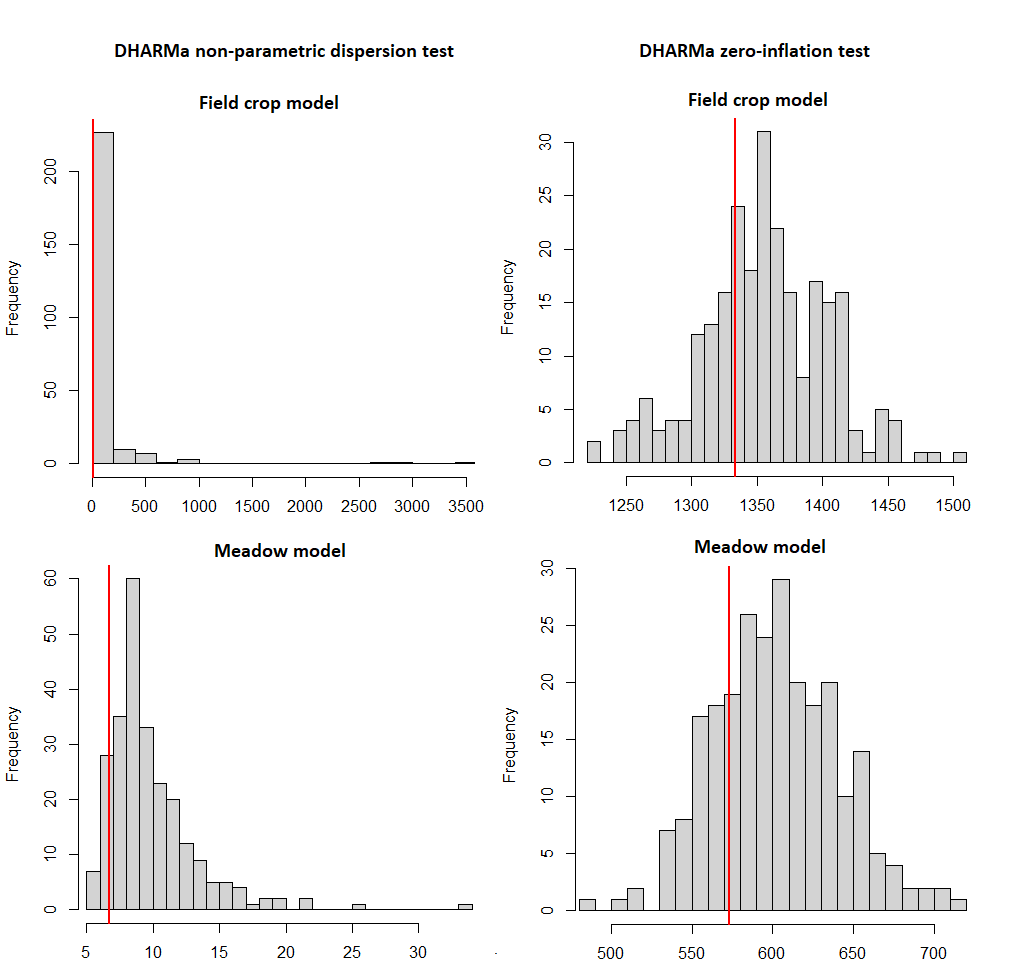
\includegraphics[width=1\linewidth]{solitary_bees_files/figure-latex/residual-sb.png} \caption{Residual diagnostics for solitary bee models, made with \emph{DHARMa} package (Hartig, \protect\hyperlink{ref-dharma2020}{2020}). Grey bars are simulated values, red line is fitted model.}\label{fig:residualsdiag}
\end{figure}

\clearpage

\hypertarget{appendix-d}{%
\section{Appendix D}\label{appendix-d}}

To detect the presence of temporal autocorrelation in the residuals, we
applied the Durbin Watson test to the sites which were monitored at
least three consecutive years. Thus, we could test 393 plot/year couples
over 767.

\begin{figure}[H]
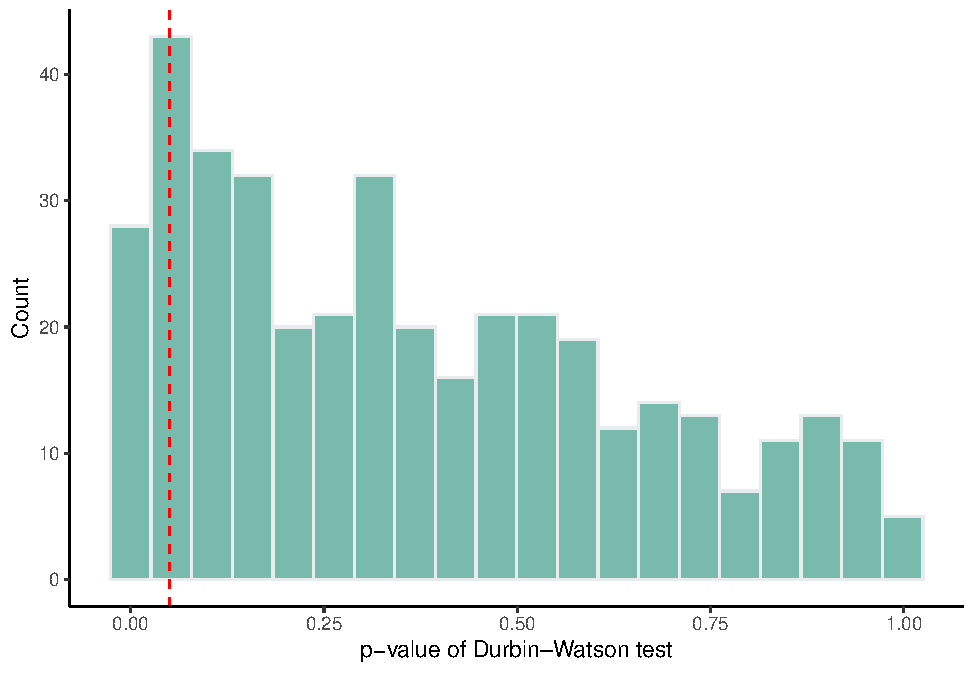
\includegraphics[width=1\linewidth]{solitary_bees_files/figure-latex/autocor} \caption{Distribution of Durbin-Watson test p-values, for residuals of fieldcrop edge model. Red dashed line is the 0.05 threshold.}\label{fig:DW}
\end{figure}

51 plot/year couples have a p-value lower than 0.05. It's only 6.65\% of
plot/year couples.


\bibliographystyle{spphys}
\bibliography{bibliography.bib}

\end{document}
